\newpage
\section{Aufgabe 3}
Im Rahmen dieser Aufgabe wird die Schallgeschwindigkeit in einem Metall bestimmt, indem ein Metallstab so eingespannt wird, das nur eine Schwingmode auftritt.
\subsection{Aufbau}
Der Aufbau gestaltet sich in diesem Fall relativ einfach. Die Metallstäbe werden so in Stative eingespannt, dass entweder nur die \(n=1\)- oder die \(n=2\)-Mode angeregt werden kann. Für die \(n=1\)-Mode ist das die Mitte des Stabs und für die \(n=2\)-Mode die Punkte bei \(\frac{1}{4}\) und \(\frac{3}{4}\). Um die Schwingfrequenz zu messen wird ein Mikrophon an den Stab postiert und an das Computer-Oszilloskop angeschlossen.
\subsection{Fehlerabschätzung}
\subsection{Gegebenes}
Gegeben sind die Längen und dichten der Stäbe mit:
\begin{center}
\begin{tabular}{c|c}
Größe & Wert\\\hline
\(l_{Stahl}\) & \((149,95 \pm 0,1)\,cm\) \\
\(l_{Messing}\) & \((146,35 \pm 0,1)\,cm\) \\
\(\rho_{Stahl}\) & \((7,5 \pm 0,3)\,\cdot 1000\frac{kg}{m^3}\) \\
\(\rho_{Messing}\) & \((8,4 \pm 0,1)\,\cdot 1000\frac{kg}{m^3}\)
\end{tabular}
\captionof{table}{Gegebene Daten der Metallstäbe}
\end{center}
\subsection{Kurven und Messwerte} Gemessen wurde die Frequenz indem die Schwingungen pro Zeitintervall ermittelt wurden. Beispielhaft sieht das so aus:
\begin{center}
\noindent
\begin{minipage}{\linewidth}
\centering
\makebox[0cm]{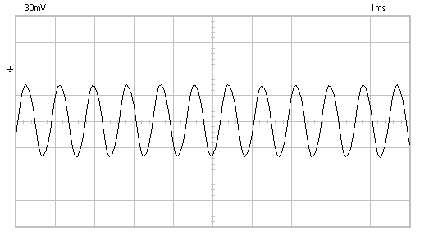
\includegraphics[width=\textwidth]{graphen/a3/Messing_1_1}}
\captionof{figure}{Frequnz Messingstab in der \(n=1\)-Mode}
\end{minipage}
\end{center}
\begin{equation}
\Rightarrow f = \frac{n}{\Delta T} \approx \frac{7}{6ms} = 1166\, Hz \notag
\end{equation}
So wurden folgende Frequenzen ermittelt:
\begin{center}
\begin{tabular}{c|c|c}
Mode \(n\) & \(f\, [Hz]\) Messing & \(f\, [Hz]\) Stahl \\\hline
1 & 1200 & 1633 \\
1 & 1166 & 1600 \\
2 & 2308 & 3269 \\
2 & 2353 & 3269
\end{tabular}
\end{center}
\subsection{Graphen}
Um diese Auswerten zu können werden diese geplottet und mit einer Ursprungsgeraden gefittet.
\begin{center}
\noindent
\begin{minipage}{\linewidth}
\centering
\makebox[0cm]{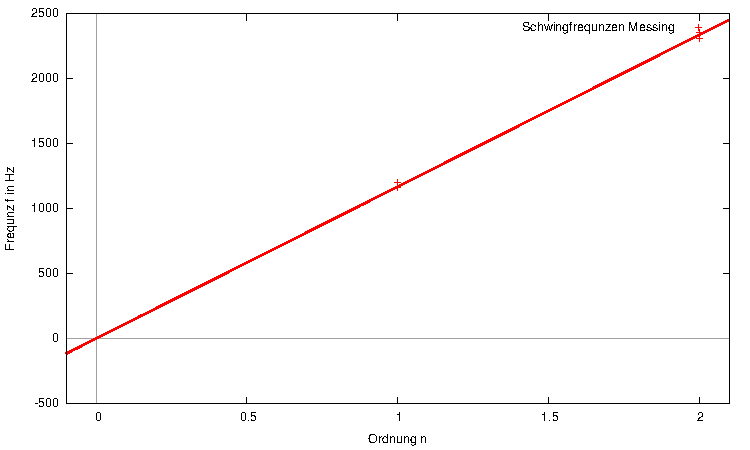
\includegraphics[width=\textwidth]{graphen/gnuplot/a3m}}
\captionof{figure}{Frequnzen beim Messingstab}
\end{minipage}
\end{center}
\begin{center}
\noindent
\begin{minipage}{\linewidth}
\centering
\makebox[0cm]{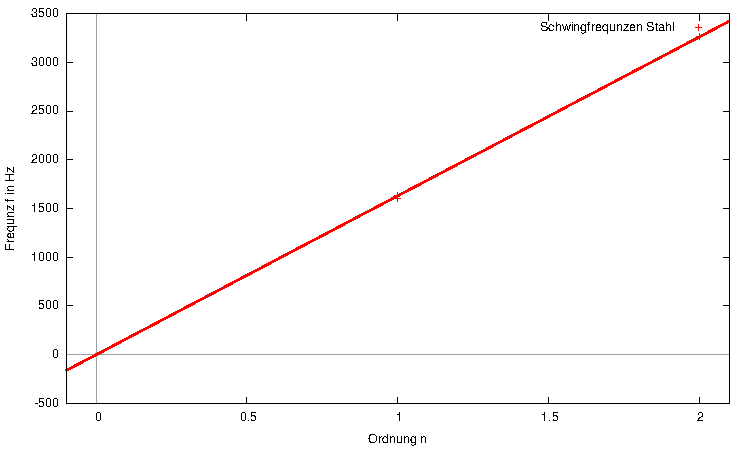
\includegraphics[width=\textwidth]{graphen/gnuplot/a3s}}
\captionof{figure}{Frequnzen beim Stahlstab}
\end{minipage}
\end{center}
Die lineare Regression ergab folgende Steigungen:
\begin{align}
b_{Messing} = (1168,8 \pm 8,4)\, Hz \notag \\
b_{Stahl} = (1630,9 \pm 5,9)\, Hz \notag
\end{align}
\subsection{Auswertung}
Da die Moden der Stäbe offenen Enden entsprechen gilt wie in Aufgabe 2 auch hier:
\begin{equation}
f(n) = n \cdot \frac{c}{2l}
\end{equation}
Daher kann die Steigung identifiziert werden um \(c\) zu bestimmen:
\begin{align}
b &= \frac{c}{2l}\\
\Rightarrow c &= b \cdot 2l\\
\Delta c &= c \cdot \sqrt{\left( \frac{\Delta b}{b} \right)^2+ \left( \frac{\Delta l}{l} \right)^2}\\
c_{Messing} &= (3421 \pm 25)\, \frac{m}{s} \notag \\
c_{Stahl} &=  (4891 \pm 18)\, \frac{m}{s} \notag
\end{align}
Um daraus das Elastizitätsmodul \(E\) zu errechnen \eqref{c} verwendet, für einen Festkörper gilt \(D = E\):
\begin{align}
c^2 &= \frac{E}{\rho} \\
\Rightarrow E &= c^2 \cdot \rho \\
\Delta E &= E \cdot \sqrt{\left(\frac{2\Delta c}{c}\right)^2+\left(\frac{\Delta \rho}{\rho}\right)^2 }\\
E_{Messing} &= (98,3 \pm 1,6) \, \frac{kN}{mm^2} \notag \\
E_{Stahl} &= (179,4 \pm 7,3) \, \frac{kN}{mm^2} \notag
\end{align}
\subsection{Fazit und Vergleich}
Auch dieser Versuch war sehr einfach durchführbar. Die Messung war sogar relativ genau und qualitativ stimmt die Messung mit den Erwartungen überein, da Die Werte zu einer Ursprungsgeraden passen. Ein Vergleich mit Literaturwerten ist schwierig, da sowohl die Schallgeschwindigkeiten, als auch die Elastizitätsmodule stark von der genauen Legierung abhängen. Eine Gegenüberstellung soll dennoch nicht ausbleiben:
\begin{center}
\begin{tabular}{c|c|c|c}
Größe & Messung & Literatur\\\hline
\(c_{Messing}\) & \((3420 \pm 30)\, \frac{m}{s}\) & \(3500\, \frac{m}{s}\)\\
\(c_{Stahl}\) & \((4890 \pm 20)\, \frac{m}{s}\) & \(4900\, \frac{m}{s}\)\\
\(E_{Messing}\) & \((98 \pm 2) \, \frac{kN}{mm^2}\) & \(78-123 \, \frac{kN}{mm^2}\) \\
\(E_{Stahl}\) & \((179 \pm 8) \, \frac{kN}{mm^2}\) & \(195-210 \, \frac{kN}{mm^2}\)
\end{tabular}
\end{center}
Die Ermittelten Werte sind also sehr nahe an Literaturwerten ähnlicher Metalle. Es ist somit nicht davon auszugehen, dass die Messung nicht erfolgreich verlaufen ist.